
%% bare_conf.tex
%% V1.4b
%% 2015/08/26
%% by Michael Shell
%% See:
%% http://www.michaelshell.org/
%% for current contact information.
%%
%% This is a skeleton file demonstrating the use of IEEEtran.cls
%% (requires IEEEtran.cls version 1.8b or later) with an IEEE
%% conference paper.
%%
%% Support sites:
%% http://www.michaelshell.org/tex/ieeetran/
%% http://www.ctan.org/pkg/ieeetran
%% and
%% http://www.ieee.org/

%%*************************************************************************
%% Legal Notice:
%% This code is offered as-is without any warranty either expressed or
%% implied; without even the implied warranty of MERCHANTABILITY or
%% FITNESS FOR A PARTICULAR PURPOSE! 
%% User assumes all risk.
%% In no event shall the IEEE or any contributor to this code be liable for
%% any damages or losses, including, but not limited to, incidental,
%% consequential, or any other damages, resulting from the use or misuse
%% of any information contained here.
%%
%% All comments are the opinions of their respective authors and are not
%% necessarily endorsed by the IEEE.
%%
%% This work is distributed under the LaTeX Project Public License (LPPL)
%% ( http://www.latex-project.org/ ) version 1.3, and may be freely used,
%% distributed and modified. A copy of the LPPL, version 1.3, is included
%% in the base LaTeX documentation of all distributions of LaTeX released
%% 2003/12/01 or later.
%% Retain all contribution notices and credits.
%% ** Modified files should be clearly indicated as such, including  **
%% ** renaming them and changing author support contact information. **
%%*************************************************************************


% *** Authors should verify (and, if needed, correct) their LaTeX system  ***
% *** with the testflow diagnostic prior to trusting their LaTeX platform ***
% *** with production work. The IEEE's font choices and paper sizes can   ***
% *** trigger bugs that do not appear when using other class files.       ***                          ***
% The testflow support page is at:
% http://www.michaelshell.org/tex/testflow/



\documentclass[conference]{IEEEtran}
% Some Computer Society conferences also require the compsoc mode option,
% but others use the standard conference format.
%
% If IEEEtran.cls has not been installed into the LaTeX system files,
% manually specify the path to it like:
% \documentclass[conference]{../sty/IEEEtran}





% Some very useful LaTeX packages include:
% (uncomment the ones you want to load)


% *** MISC UTILITY PACKAGES ***
%
%\usepackage{ifpdf}
% Heiko Oberdiek's ifpdf.sty is very useful if you need conditional
% compilation based on whether the output is pdf or dvi.
% usage:
% \ifpdf
%   % pdf code
% \else
%   % dvi code
% \fi
% The latest version of ifpdf.sty can be obtained from:
% http://www.ctan.org/pkg/ifpdf
% Also, note that IEEEtran.cls V1.7 and later provides a builtin
% \ifCLASSINFOpdf conditional that works the same way.
% When switching from latex to pdflatex and vice-versa, the compiler may
% have to be run twice to clear warning/error messages.






% *** CITATION PACKAGES ***
%
%\usepackage{cite}
% cite.sty was written by Donald Arseneau
% V1.6 and later of IEEEtran pre-defines the format of the cite.sty package
% \cite{} output to follow that of the IEEE. Loading the cite package will
% result in citation numbers being automatically sorted and properly
% "compressed/ranged". e.g., [1], [9], [2], [7], [5], [6] without using
% cite.sty will become [1], [2], [5]--[7], [9] using cite.sty. cite.sty's
% \cite will automatically add leading space, if needed. Use cite.sty's
% noadjust option (cite.sty V3.8 and later) if you want to turn this off
% such as if a citation ever needs to be enclosed in parenthesis.
% cite.sty is already installed on most LaTeX systems. Be sure and use
% version 5.0 (2009-03-20) and later if using hyperref.sty.
% The latest version can be obtained at:
% http://www.ctan.org/pkg/cite
% The documentation is contained in the cite.sty file itself.






% *** GRAPHICS RELATED PACKAGES ***
%
\ifCLASSINFOpdf
  % \usepackage[pdftex]{graphicx}
  % declare the path(s) where your graphic files are
  % \graphicspath{{../pdf/}{../jpeg/}}
  % and their extensions so you won't have to specify these with
  % every instance of \includegraphics
  % \DeclareGraphicsExtensions{.pdf,.jpeg,.png}
\else
  % or other class option (dvipsone, dvipdf, if not using dvips). graphicx
  % will default to the driver specified in the system graphics.cfg if no
  % driver is specified.
  % \usepackage[dvips]{graphicx}
  % declare the path(s) where your graphic files are
  % \graphicspath{{../eps/}}
  % and their extensions so you won't have to specify these with
  % every instance of \includegraphics
  % \DeclareGraphicsExtensions{.eps}
\fi
% graphicx was written by David Carlisle and Sebastian Rahtz. It is
% required if you want graphics, photos, etc. graphicx.sty is already
% installed on most LaTeX systems. The latest version and documentation
% can be obtained at: 
% http://www.ctan.org/pkg/graphicx
% Another good source of documentation is "Using Imported Graphics in
% LaTeX2e" by Keith Reckdahl which can be found at:
% http://www.ctan.org/pkg/epslatex
%
% latex, and pdflatex in dvi mode, support graphics in encapsulated
% postscript (.eps) format. pdflatex in pdf mode supports graphics
% in .pdf, .jpeg, .png and .mps (metapost) formats. Users should ensure
% that all non-photo figures use a vector format (.eps, .pdf, .mps) and
% not a bitmapped formats (.jpeg, .png). The IEEE frowns on bitmapped formats
% which can result in "jaggedy"/blurry rendering of lines and letters as
% well as large increases in file sizes.
%
% You can find documentation about the pdfTeX application at:
% http://www.tug.org/applications/pdftex





% *** MATH PACKAGES ***
%
\usepackage{amsmath}
\usepackage{url}
% A popular package from the American Mathematical Society that provides
% many useful and powerful commands for dealing with mathematics.
%
% Note that the amsmath package sets \interdisplaylinepenalty to 10000
% thus preventing page breaks from occurring within multiline equations. Use:
%\interdisplaylinepenalty=2500
% after loading amsmath to restore such page breaks as IEEEtran.cls normally
% does. amsmath.sty is already installed on most LaTeX systems. The latest
% version and documentation can be obtained at:
% http://www.ctan.org/pkg/amsmath





% *** SPECIALIZED LIST PACKAGES ***
%
%\usepackage{algorithmic}
% algorithmic.sty was written by Peter Williams and Rogerio Brito.
% This package provides an algorithmic environment fo describing algorithms.
% You can use the algorithmic environment in-text or within a figure
% environment to provide for a floating algorithm. Do NOT use the algorithm
% floating environment provided by algorithm.sty (by the same authors) or
% algorithm2e.sty (by Christophe Fiorio) as the IEEE does not use dedicated
% algorithm float types and packages that provide these will not provide
% correct IEEE style captions. The latest version and documentation of
% algorithmic.sty can be obtained at:
% http://www.ctan.org/pkg/algorithms
% Also of interest may be the (relatively newer and more customizable)
% algorithmicx.sty package by Szasz Janos:
% http://www.ctan.org/pkg/algorithmicx




% *** ALIGNMENT PACKAGES ***
%
%\usepackage{array}
% Frank Mittelbach's and David Carlisle's array.sty patches and improves
% the standard LaTeX2e array and tabular environments to provide better
% appearance and additional user controls. As the default LaTeX2e table
% generation code is lacking to the point of almost being broken with
% respect to the quality of the end results, all users are strongly
% advised to use an enhanced (at the very least that provided by array.sty)
% set of table tools. array.sty is already installed on most systems. The
% latest version and documentation can be obtained at:
% http://www.ctan.org/pkg/array


% IEEEtran contains the IEEEeqnarray family of commands that can be used to
% generate multiline equations as well as matrices, tables, etc., of high
% quality.




% *** SUBFIGURE PACKAGES ***
%\ifCLASSOPTIONcompsoc
%  \usepackage[caption=false,font=normalsize,labelfont=sf,textfont=sf]{subfig}
%\else
%  \usepackage[caption=false,font=footnotesize]{subfig}
%\fi
% subfig.sty, written by Steven Douglas Cochran, is the modern replacement
% for subfigure.sty, the latter of which is no longer maintained and is
% incompatible with some LaTeX packages including fixltx2e. However,
% subfig.sty requires and automatically loads Axel Sommerfeldt's caption.sty
% which will override IEEEtran.cls' handling of captions and this will result
% in non-IEEE style figure/table captions. To prevent this problem, be sure
% and invoke subfig.sty's "caption=false" package option (available since
% subfig.sty version 1.3, 2005/06/28) as this is will preserve IEEEtran.cls
% handling of captions.
% Note that the Computer Society format requires a larger sans serif font
% than the serif footnote size font used in traditional IEEE formatting
% and thus the need to invoke different subfig.sty package options depending
% on whether compsoc mode has been enabled.
%
% The latest version and documentation of subfig.sty can be obtained at:
% http://www.ctan.org/pkg/subfig




% *** FLOAT PACKAGES ***
%
%\usepackage{fixltx2e}
% fixltx2e, the successor to the earlier fix2col.sty, was written by
% Frank Mittelbach and David Carlisle. This package corrects a few problems
% in the LaTeX2e kernel, the most notable of which is that in current
% LaTeX2e releases, the ordering of single and double column floats is not
% guaranteed to be preserved. Thus, an unpatched LaTeX2e can allow a
% single column figure to be placed prior to an earlier double column
% figure.
% Be aware that LaTeX2e kernels dated 2015 and later have fixltx2e.sty's
% corrections already built into the system in which case a warning will
% be issued if an attempt is made to load fixltx2e.sty as it is no longer
% needed.
% The latest version and documentation can be found at:
% http://www.ctan.org/pkg/fixltx2e


%\usepackage{stfloats}
% stfloats.sty was written by Sigitas Tolusis. This package gives LaTeX2e
% the ability to do double column floats at the bottom of the page as well
% as the top. (e.g., "\begin{figure*}[!b]" is not normally possible in
% LaTeX2e). It also provides a command:
%\fnbelowfloat
% to enable the placement of footnotes below bottom floats (the standard
% LaTeX2e kernel puts them above bottom floats). This is an invasive package
% which rewrites many portions of the LaTeX2e float routines. It may not work
% with other packages that modify the LaTeX2e float routines. The latest
% version and documentation can be obtained at:
% http://www.ctan.org/pkg/stfloats
% Do not use the stfloats baselinefloat ability as the IEEE does not allow
% \baselineskip to stretch. Authors submitting work to the IEEE should note
% that the IEEE rarely uses double column equations and that authors should try
% to avoid such use. Do not be tempted to use the cuted.sty or midfloat.sty
% packages (also by Sigitas Tolusis) as the IEEE does not format its papers in
% such ways.
% Do not attempt to use stfloats with fixltx2e as they are incompatible.
% Instead, use Morten Hogholm'a dblfloatfix which combines the features
% of both fixltx2e and stfloats:
%
% \usepackage{dblfloatfix}
% The latest version can be found at:
% http://www.ctan.org/pkg/dblfloatfix




% *** PDF, URL AND HYPERLINK PACKAGES ***
%
%\usepackage{url}
% url.sty was written by Donald Arseneau. It provides better support for
% handling and breaking URLs. url.sty is already installed on most LaTeX
% systems. The latest version and documentation can be obtained at:
% http://www.ctan.org/pkg/url
% Basically, \url{my_url_here}.




% *** Do not adjust lengths that control margins, column widths, etc. ***
% *** Do not use packages that alter fonts (such as pslatex).         ***
% There should be no need to do such things with IEEEtran.cls V1.6 and later.
% (Unless specifically asked to do so by the journal or conference you plan
% to submit to, of course. )


% correct bad hyphenation here
\hyphenation{op-tical net-works semi-conduc-tor}

\usepackage{graphicx}
\graphicspath{{img/}}

\begin{document}
%
% paper title
% Titles are generally capitalized except for words such as a, an, and, as,
% at, but, by, for, in, nor, of, on, or, the, to and up, which are usually
% not capitalized unless they are the first or last word of the title.
% Linebreaks \\ can be used within to get better formatting as desired.
% Do not put math or special symbols in the title.
\title{Game, Set, Learn: A Machine Learning Approach to Tennis Match Prediction}


% author names and affiliations
% use a multiple column layout for up to three different
% affiliations
\author{\IEEEauthorblockN{Nikhil Shenoy}
% \IEEEauthorblockA{School of Electrical and\\Computer Engineering\\
% Georgia Institute of Technology\\
% Atlanta, Georgia 30332--0250\\
% Email: http://www.michaelshell.org/contact.html}
\and
\IEEEauthorblockN{Claire Wang}
% \IEEEauthorblockA{Twentieth Century Fox\\
% Springfield, USA\\
% Email: homer@thesimpsons.com}
\and
\IEEEauthorblockN{Abhinav Malik}}
% \IEEEauthorblockA{Starfleet Academy\\
% San Francisco, California 96678--2391\\
% Telephone: (800) 555--1212\\
% Fax: (888) 555--1212}}

% conference papers do not typically use \thanks and this command
% is locked out in conference mode. If really needed, such as for
% the acknowledgment of grants, issue a \IEEEoverridecommandlockouts
% after \documentclass

% for over three affiliations, or if they all won't fit within the width
% of the page, use this alternative format:
% 
%\author{\IEEEauthorblockN{Michael Shell\IEEEauthorrefmark{1},
%Homer Simpson\IEEEauthorrefmark{2},
%James Kirk\IEEEauthorrefmark{3}, 
%Montgomery Scott\IEEEauthorrefmark{3} and
%Eldon Tyrell\IEEEauthorrefmark{4}}
%\IEEEauthorblockA{\IEEEauthorrefmark{1}School of Electrical and Computer Engineering\\
%Georgia Institute of Technology,
%Atlanta, Georgia 30332--0250\\ Email: see http://www.michaelshell.org/contact.html}
%\IEEEauthorblockA{\IEEEauthorrefmark{2}Twentieth Century Fox, Springfield, USA\\
%Email: homer@thesimpsons.com}
%\IEEEauthorblockA{\IEEEauthorrefmark{3}Starfleet Academy, San Francisco, California 96678-2391\\
%Telephone: (800) 555--1212, Fax: (888) 555--1212}
%\IEEEauthorblockA{\IEEEauthorrefmark{4}Tyrell Inc., 123 Replicant Street, Los Angeles, California 90210--4321}}




% use for special paper notices
%\IEEEspecialpapernotice{(Invited Paper)}




% make the title area
\maketitle

% As a general rule, do not put math, special symbols or citations
% in the abstract
\begin{abstract}
    Tennis is an international sport that people enjoy watching for the variety of style, strategies against different players when playing on different surfaces, and the globe-trotting part of the ATP World Tour. With an increasingly talented group of players at the top of the game, a strong incentive exists, in the betting and purely academic arenas, to predict the outcome of matches. In this project, we seek to use machine learning methods to build a model of a match-up between two players based on statistics about their playing style, and predict the winner of the match. By doing this repeatedly on a tournament draw, we aim to construct a model of which statistics are most important in determining the winner of a match. We limit the scope of our model to the ATP World Tour, which is top level of the men’s game.
\end{abstract}

% no keywords




% For peer review papers, you can put extra information on the cover
% page as needed:
% \ifCLASSOPTIONpeerreview
% \begin{center} \bfseries EDICS Category: 3-BBND \end{center}
% \fi
%
% For peerreview papers, this IEEEtran command inserts a page break and
% creates the second title. It will be ignored for other modes.
\IEEEpeerreviewmaketitle



\section{Introduction}
% no \IEEEPARstart
Models for match prediction are useful for a variety of parties. Coaches can use the information to determine where their player is weak and improve those aspects of their game. In the betting world, predictions can be used to place bets on favorite players for big cash payoffs. Even the players themselves can use such a model to assess a matchup with an upcoming opponent, and what their chance is to get to a certain round in the draw. All of these stakeholders can also use the model to analyze what went wrong in matches that were considered upsets, such as Roger Federer, a seven-time Wimbledon champion, losing to Sergiy Stakhovsky in the second round of Wimbledon 2013. Our goal in this project is to create a model that can account for all of these situations and provide useful information to all interested parties.

% The objective of our project is to predict match results given two players’ statistics collected from each of their match history, evaluate the performance of our models by their accuracy, precision, recall and f1 score, and analyse how to extract features to solve problems like unseen examples, bias in number of training examples and etc. and how those issues affect our models’ performance. In the process of feature analysis, we would also like to compare our models’ performance with existing models’ performances, thus analysing how much the extracted features contributed to each model.  
% There are a variety of sources for tennis data, but we found that the most comprehensive and attribute-rich data set comes from a Github repository created by Jeff Sackman \cite{sackmann}. This data set consists of many important attributes about a match-up such as the court surface, the player’s seed in the tournament, serve percentages, and so on. Additionally, the repository has collected data from every season from the year 2000 to the current season, which gives us plenty of data to work with.
% You must have at least 2 lines in the paragraph with the drop letter
% (should never be an issue)

\section{Previous Work}
A plethora of work has been done on tournament predictions, and tennis predictions in specific. Due to the nature of the hierarchical scoring system in tennis (4 points in a game, 6 games in a set, win ⅔ or ⅗ sets, with variations), structured models are easier to create as opposed to other sports. Additionally, papers have been published about specific properties of the game that we can leverage  when building our model. In the first paper we looked at, written by Klaassen and Magnus \cite{iid_points}, the authors analyze whether individual points in tennis are independently and identically distributed. They concluded that points are neither independent of each other nor identically distributed;however, they also concluded that deviations are sufficiently small that the IID hypothesis will still provide a good approximation. This fact is extremely useful as it allows us to build models without needing to continuously look at the previous state of a match.
Sipko \cite{sipko} has also done extensive analysis of similar data, and provides a reference for feature extraction and results from models he has tried. One method Sipko uses for feature extraction when comparing two players is to consider a set of common opponents between two players. For a specific raw attribute, such as the percentage of points won when returning serve,  and a matchup between Player 1 and Player 2, the value of the attribute is measured between Player 1 and every player in the set of common opponents. The process is repeated for Player 2. Then, the vectors for each player are averaged to generate two scores. These scores can then be used to compare the performance of Player 1 versus Player 2 for this specific attribute. By using this method as one of our feature extractors, we can build much more nuanced models.


\section{Methodology}
	Our experiments seek to answer three questions:

		\begin{enumerate}
			\item Are machine learning models better at predicting match results than a casual watcher using basic rules of thumb?
			\item Which machine learning model is the best for prediction?
			\item Which are the most important features to consider when predicting a match?
		\end{enumerate}

	In the first question, we assess whether machine learning models will actually do better than a casual fan using his own instincts. It is very common for a fan to say ``this player is ranked higher than his opponent, so I think he will win'', and use no other data for his prediction. We turn this statements into baselines, or rules of thumb, to simulate the performance of a ``fan classifier''. We compare the results against machine learning models to determine whether advanced analysis of tennis data is really useful.

	We expect that machine learning methods will do better than a simple baseline, so the next question we consider is which model to choose. Many classifiers have been created over the years, and we compare the support vector machine, neural networks, and logistic regression to try and find the best model that suits this particular problem. We will compare the accuracy of each model on a test data set to determine the best model.

	Finally, once we have the best model, we attempt to discover the most important features of a match. Such information is useful to the stakeholders because it simplifies the problem of predictions into a handful of statistics that they can use to improve their game or maximize their winnings. To do this, we perform an ablation study to analyze the effect of removing certain features from the classification.

	We decided to use tennis tournament data from a repository created by Jeff Sackmann \cite{sackmann}, which contains all data in ATP matches from 1968 to 2017. In each match, a number of statistics such as the number of aces, double faults, and break points saved, are detailed for each player. These statistics provide ample information about the match that our classifiers can train on. 

% We train our models first on the raw data, using existing attributes as features and predict results and collect performance data on each model. Then we will extract new sets of features from the raw attributes based on the methods mentioned in \cite{sipko}. One potential challenge which is also mentioned in the paper is that the data set only contains statistics for paired players in previous matches, if two players have never been matched together, then we have no training sets to predict on, and in this situation, we will extract higher level data based on common opponents, so that our models will be able to predict even on unseen examples. For bias in number of training examples for each player, we think assigning a feature type which reflects a player’s number of past matches would help weighing the model accordingly. 
% The models we choose to use are SVM and online algorithms. We chose those two models because in assignment 2, we have experimented and studied them extensively, and it would be interesting to see how they perform on a different set of real world data. SVM is used in multiple existing models, and it would be more convenient for us to do feature analysis when comparing results from the same model. 


\section{Data Preprocessing}
We used a variety of techniques to prepare our data for input into the algorithm. First we checked for the unique values for each feature in the raw data, and removed examples where the value would be unusable in our feature extraction phase. An example of this would be finding ``nan'' values in the numerical features; performing any operations on data with this value would result in a value that our classifiers would not be able to process. We considered techniques on how best to replace the value, but we eventually decided that the schemes we had come up with could still alter the outcome of the classification. Thus, we decided to drop the inconsistent examples entirely.

We also restricted the data that we considered to the years 2000-2017. Sackmann's repository contained a wealth of tennis data going back to the inception of the ATP World Tour in 1968, but we decided not to use all of the data because of how the game has evolved since then. There are a number of issues that would have cropped up if we had used the full data set:

\begin{itemize}
	\item \textbf{Too much data:} While we would have liked to use the full set, we did not have the computational power to do our feature extraction in a reasonable amount of time. Our feature extraction methods (as will be discussed in the next section) tend to be $O(n^2)$ operations, and they would have become prohibitively expensive when working with $O(100000)$ examples.
	\item \textbf{Difference in technology:} The racquets, shoes, court surface, and ball, among other items, have changed drastically over the years, allowing some players to excel.For example, racquets have allowed players in the last 20 years to hit harder and with more spin, which was not possible before. To avoid this, we limit the years considered so that the issue of varied sports technology is relatively constant.
	\item \textbf{Difference in playing style:} From the year 1968 to around the middle of the 1990s, the playing style for most tennis players was ``serve-and-volley''. After that period of time, players began to finish more points at the baseline, resulting in the playing style we have today. This difference prioritizes certain statistics, like serves and volleys, more than others such as statistics. We eliminate this particular difference by choosing an era with consistent playing style.
\end{itemize}

Another decision was made to remove all the Davis Cup matches from the data set. The Davis Cup format requires players to be on a team and represent their country, while countries face each other in a tournament for the final prize. This format has different rules than normal singles plays, as each team has a captain and can decide who plays at what spot in their lineup against another country. Since these matches can be arranged differently than a standard tournament draw, we consider it as noise and remove all non-ATP matches.

Finally, we turned the original data set into a binary classification problem. The raw data set had the two players' statistics and the name of the winner, which isn't an easy format to work with. Instead, we labeled the players ``Player 1`` and ``Player 2``, and then added a label column such that the value would be 1 if ``Player 1`` won the match and zero otherwise. By doing this, the question our classifiers seek to answer is ``what are the weights of the features that will help Player 1 win the match?'', which is an easier problem to solve.

\section{Feature Extraction}
We used four different methods to extract features for our problem. After all the features are extracted, we create a feature vector with a length equal to the number of features, and have the aforementioned Player 1 win/loss value as our label. We provide a summary of our feature extraction methods here.

	% Symmetry
	\subsection{Symmetry of Features}
	In the original data, we are provided with two values per statistic in every example. For example, the ``aces'' statistic is recorded for both Player 1 and Player 2. This representation provides us with specific information for each player, but it also has a drawback; if we exchanged the labels for Player 1 and Player 2, then our classifier could assign different weights to the individual feature and predict a different outcome. To avoid this, we create a single feature with the raw statistics as shown in Equation \ref{symmetry}.

	\begin{equation} \label{symmetry}
		\text{Feature}_{i} = \text{Raw}_{1,i} - \text{Raw}_{2,i}
	\end{equation}

	where $i$ is the example index, $\text{RAW}$ is the raw feature from the original data set, and $\text{FEATURE}$ is our newly generated feature. Previous work by Clark and Dyte \cite{clark_and_dyte} have shown that this representation is effective, so we transform all of our raw features using this method.

	% Common Opponent
	\subsection{Common Opponent Model}
		We also use a method called the Common Opponent Model, which was originally proposed by Knottenbelt \cite{common_opponent_model}. In this model, we consider the set of common opponents that both Player 1 and Player 2 have played against. For each of Player 1 and 2, we find the mean of the statistic against each player in the set of common opponents. Finally, we create a difference variable using the two means. 

	\begin{figure}[h]
		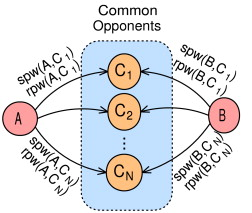
\includegraphics[scale=1.00]{common_opponent_model} % Scale included just in case we want to scale the image down
		\label{fig:common_opponent_model}
		\centering
		\caption{The Common Opponent Model}
	\end{figure}

	The idea behind this model is that comparing statistics between two players becomes more meaningful when judged against a standard baseline. We get a better idea of the true value of the statistic for each Player since we take into account his performance against a variety of opponents. All of our numerical features were calculated in this way.


	% Derived Features
	\subsection{Derived Features}
	We created derived features as a function of other features that we have. One noteable example is the Completeness feature. In debates about who the best player of all time is, commentators require that a player have a good serve, good groundstrokes, good returns, and good movement, among other factors. Someone who has all of these factors is considered a ``complete'' player. We try to simulate completeness in Equation \ref{completeness} by taking the product of the first serves won, the second serves won, and the fraction of break points won. Unfortunately, our data set did not have information about groundstrokes and court movement, so we limited the definition to just three component features.

	\begin{equation} \label{completeness}
		\text{Completeness}_{i} = \text{1stWon}_{i} * \text{2ndWon}_{i} * \frac{\text{bpSaved}_{i}}{\text{bpFaced}_{i}}
	\end{equation}

	By multiplying the component features, we generate a derived feature that requires a player to be competent in all areas for the feature to be significant. But if any is lacking, then the feature value will decrease and potentially not have as much impact on the final prediction. We feel that such features provide additional information about the problem based on domain-specific knowledge and can bolster the accuracy of our models.

	% Categorical variables
	\subsection{Categorical Features}
	While the idea of categorical variables is not new, we use it to include information that was not used in previous work. These works always included statistics about a player's performance, but never included information about the surface of the court. Tennis is played on four types of surfaces; hard, grass, clay, and carpet. The tactics used to win are different on each surface, and some players' styles are more suited to one surface than another. To account for the court surface in our feature vector, we use a 1-Hot encoding to indicate which type of surface a particular match is played on.

\section{Experiments}
Our experiments seek to answer the three questions we set in the beginning of the project:

	\begin{enumerate}
		\item Are machine learning models better at predicting match results than a casual watcher using basic rules of thumb?
		\item Which machine learning model is the best for prediction?
		\item Which are the most important features to consider when predicting a match?
	\end{enumerate}

We briefly describe the models that we use, and then detail the results of our experiments.

	\subsection{Models}

		\subsubsection{Support Vector Machines}
		We chose to use a Support Vector Machine (SVM) for classification for two main reasons; first, no previous published work has utilized the SVM for this problem, and we saw an opportunity to examine how effective this classifier is. Also, the SVM does not encounter local minima during the calculation, which provides an advantage over classifiers like neural networks. We used the Soft SVM formulation in Equation \ref{soft_svm} to build the classifier, where $w$ is the weight vector, $y_{i}$ is the label of example $i$, $x_{i}$ is the $i$-th example, and $C$ is a hyperparameter that scales the penalty of performing misclassifications.

		\begin{equation} \label{soft_svm}
				\min_{w} \frac{1}{2}w^{T}w + C \sum_{i} \max(0, 1-y_{i}w^{T}x_{i})
		\end{equation}

		To find the optimal hyperparameters for the SVM, we used a grid search over three kernels (linear, polynomial, and the radial basis function) and the scaling factor $C$. We trained on our training set and tested on the validation set, giving the results in Table \ref{svm_grid_search}.

		\begin{table}[h!]
		\centering
		\begin{tabular}{| c | c | c |}
		\hline
		\textbf{Kernel} & $C$ & \textbf{Accuracy} \\
		\hline
		Linear & 0.25 & .867 \\
		\hline
		Linear & 0.5 & .871 \\
		\hline
		Linear & 1.0 & .870 \\
		\hline
		Linear & 10 & .869 \\
		\hline
		Polynomial & 0.25 & .859 \\
		\hline
		Polynomial & 0.5 & .860 \\
		\hline
		Polynomial & 1.0 & .861 \\
		\hline
		Polynomial & 10 & .864 \\
		\hline
		RBF & 0.25 & .864 \\
		\hline
		RBF & 0.5 & .867 \\
		\hline
		RBF & 1.0 & .864 \\
		\hline
		RBF & 10 & .861 \\
		\hline
		\end{tabular}
		\caption{Results from Tuning SVM Hyperparameters}
		\label{svm_grid_search}
		\end{table}

		From this grid search experiment, we found that the Linear Kernel with $C = 0.5$ was the optimal pair of hyperparameters for our model.

		\subsubsection{Multi-Layer Perceptron}
		A multi-layer perceptron neural network is chosen as one of the three machine learning models because we learned about perceptron in class, and different from online model, multi-layer perceptron has a non-linear activation layer that is more suited for high dimensionality and linearly inseparable features. The multi-layer perceptron we used is implemented in sklearn, and has one input layer, one hidden layer with a hundred units and one output layer.
		
		\begin{figure}[h]
		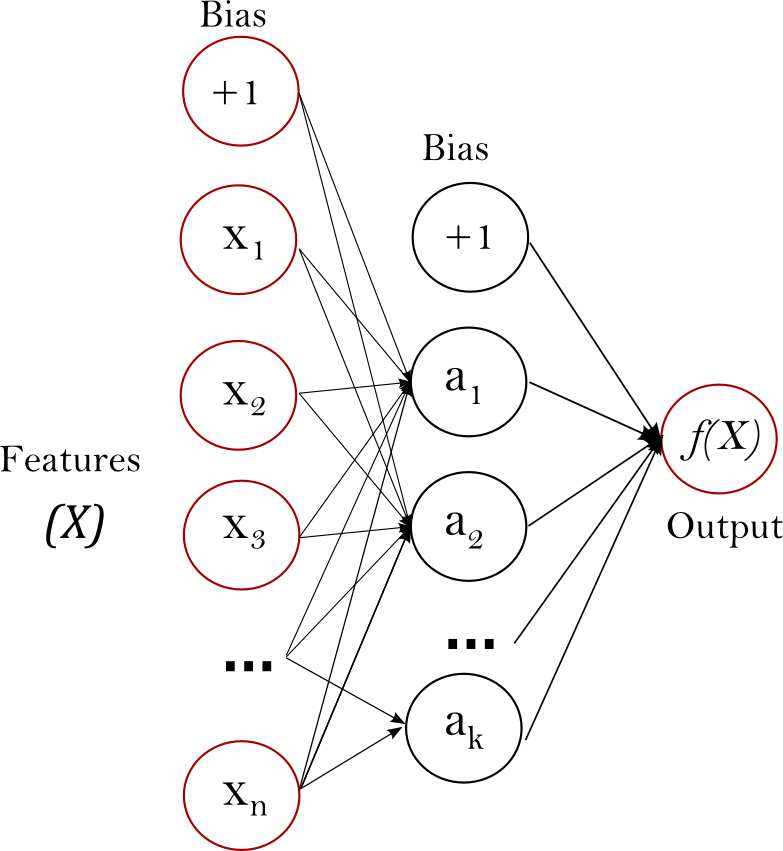
\includegraphics[scale=0.3]{mlp} % Scale included just in case we want to scale the image down
		\label{fig:multi-layer perceptron}
		\centering
		\caption{Multi-Layer Perceptron Model}
		\end{figure}

	\subsection{Ablation Study}
	To find out what the most important features in determining match outcome are, we perform an ablation study. In such a study, we first get the accuracy of the classifier with all features included. Then, we remove features one at a time, to examine the contribution each feature has to the final accuracy of the model. We performed this technique on all of our models (ACTUALLY NEED TO DO THIS FOR MLP AND LR), with results from the ablation study on our SVM shown in Figure \ref{fig:svm_ablation}.

	\begin{figure}[h]
		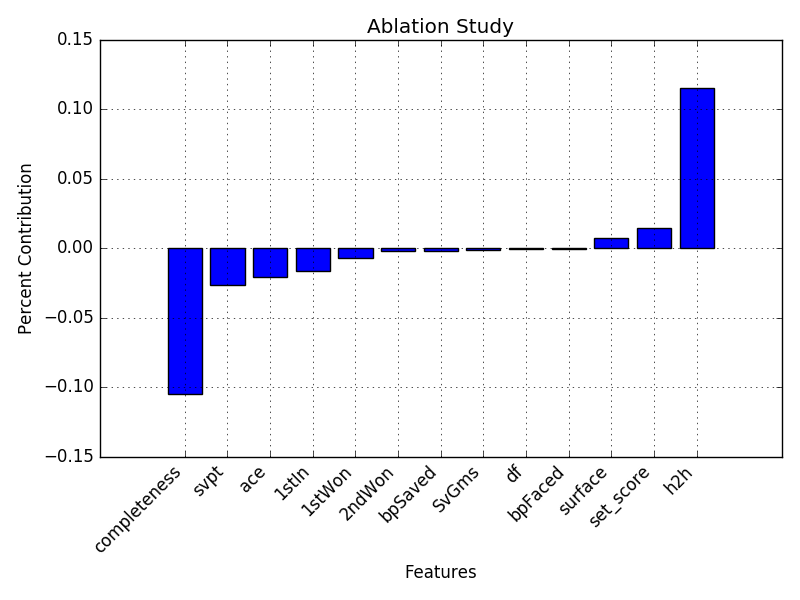
\includegraphics[scale=0.45]{svm_ablation} % Scale included just in case we want to scale the image down
		\label{fig:svm_ablation}
		\centering
		\caption{Ablation Study with SVM}
	\end{figure}

	The results from this study are interesting because of the signifiance placed on certain features. We observed that the Head-to-Head feature had the most significant contribution to the test accuracy, boosting it by about 12\%. The implication of this is that the history of the pair's past matches outweigh any of the statistics gathered during the current match. The next two most significant features were the set score and the court surface. Intuitively, the court surface must have significance due to the way the ball bounces on different material. But the more interesting trend is that the remainder of the features that we used either did not contribute to the test accuracy or actually hindered the result. From this, a conclusion is that our model provides no information about which match statistic a player should prioritize in order to win, implying that so long as the player can win, he can play whichever way he likes. The most notable of the remaining features is completeness, which is one of the derived features that we created to simulate a player's ability in multiple aspects of the game. The implication from the study is that a player training to be good at each type of shot is actually detrimental to his success, allowing one to conclude that that a player should only focus on improving certain shots, perhaps those he has a natural talent for, to increase his chances of winning. 
	We had expected the ablation study to show that each of the match statistics contributed some positive percentage to the test accuracy an dsuggest what areas a player should focus on improving. The final results, however, was that the most important feature in determining match outcome is the past Head-to-Head history and the court surface for the match.
% An example of a floating figure using the graphicx package.
% Note that \label must occur AFTER (or within) \caption.
% For figures, \caption should occur after the \includegraphics.
% Note that IEEEtran v1.7 and later has special internal code that
% is designed to preserve the operation of \label within \caption
% even when the captionsoff option is in effect. However, because
% of issues like this, it may be the safest practice to put all your
% \label just after \caption rather than within \caption{}.
%
% Reminder: the "draftcls" or "draftclsnofoot", not "draft", class
% option should be used if it is desired that the figures are to be
% displayed while in draft mode.
%
%\begin{figure}[!t]
%\centering
%\includegraphics[width=2.5in]{myfigure}
% where an .eps filename suffix will be assumed under latex, 
% and a .pdf suffix will be assumed for pdflatex; or what has been declared
% via \DeclareGraphicsExtensions.
%\caption{Simulation results for the network.}
%\label{fig_sim}
%\end{figure}

% Note that the IEEE typically puts floats only at the top, even when this
% results in a large percentage of a column being occupied by floats.


% An example of a double column floating figure using two subfigures.
% (The subfig.sty package must be loaded for this to work.)
% The subfigure \label commands are set within each subfloat command,
% and the \label for the overall figure must come after \caption.
% \hfil is used as a separator to get equal spacing.
% Watch out that the combined width of all the subfigures on a 
% line do not exceed the text width or a line break will occur.
%
%\begin{figure*}[!t]
%\centering
%\subfloat[Case I]{\includegraphics[width=2.5in]{box}%
%\label{fig_first_case}}
%\hfil
%\subfloat[Case II]{\includegraphics[width=2.5in]{box}%
%\label{fig_second_case}}
%\caption{Simulation results for the network.}
%\label{fig_sim}
%\end{figure*}
%
% Note that often IEEE papers with subfigures do not employ subfigure
% captions (using the optional argument to \subfloat[]), but instead will
% reference/describe all of them (a), (b), etc., within the main caption.
% Be aware that for subfig.sty to generate the (a), (b), etc., subfigure
% labels, the optional argument to \subfloat must be present. If a
% subcaption is not desired, just leave its contents blank,
% e.g., \subfloat[].


% An example of a floating table. Note that, for IEEE style tables, the
% \caption command should come BEFORE the table and, given that table
% captions serve much like titles, are usually capitalized except for words
% such as a, an, and, as, at, but, by, for, in, nor, of, on, or, the, to
% and up, which are usually not capitalized unless they are the first or
% last word of the caption. Table text will default to \footnotesize as
% the IEEE normally uses this smaller font for tables.
% The \label must come after \caption as always.
%
%\begin{table}[!t]
%% increase table row spacing, adjust to taste
%\renewcommand{\arraystretch}{1.3}
% if using array.sty, it might be a good idea to tweak the value of
% \extrarowheight as needed to properly center the text within the cells
%\caption{An Example of a Table}
%\label{table_example}
%\centering
%% Some packages, such as MDW tools, offer better commands for making tables
%% than the plain LaTeX2e tabular which is used here.
%\begin{tabular}{|c||c|}
%\hline
%One & Two\\
%\hline
%Three & Four\\
%\hline
%\end{tabular}
%\end{table}


% Note that the IEEE does not put floats in the very first column
% - or typically anywhere on the first page for that matter. Also,
% in-text middle ("here") positioning is typically not used, but it
% is allowed and encouraged for Computer Society conferences (but
% not Computer Society journals). Most IEEE journals/conferences use
% top floats exclusively. 
% Note that, LaTeX2e, unlike IEEE journals/conferences, places
% footnotes above bottom floats. This can be corrected via the
% \fnbelowfloat command of the stfloats package.




\section{Conclusion}
The conclusion goes here.




% conference papers do not normally have an appendix


% use section* for acknowledgment
\section*{Acknowledgment}


The authors would like to thank...





% trigger a \newpage just before the given reference
% number - used to balance the columns on the last page
% adjust value as needed - may need to be readjusted if
% the document is modified later
%\IEEEtriggeratref{8}
% The "triggered" command can be changed if desired:
%\IEEEtriggercmd{\enlargethispage{-5in}}

% references section

% can use a bibliography generated by BibTeX as a .bbl file
% BibTeX documentation can be easily obtained at:
% http://mirror.ctan.org/biblio/bibtex/contrib/doc/
% The IEEEtran BibTeX style support page is at:
% http://www.michaelshell.org/tex/ieeetran/bibtex/
%\bibliographystyle{IEEEtran}
% argument is your BibTeX string definitions and bibliography database(s)
%\bibliography{IEEEabrv,../bib/paper}
%
% <OR> manually copy in the resultant .bbl file
% set second argument of \begin to the number of references
% (used to reserve space for the reference number labels box)
\nocite{*}
\bibliographystyle{ieeetr}
\bibliography{references}






% that's all folks
\end{document}
